\chapter{画像などの挿入}
\section{PNG・JPG画像の挿入}
このようにしてPNG画像を挿入できます。
\begin{figure}[H]
    \centering
    
\includegraphics[width=8cm]{figures/computer_man1_smile.png}
    \caption{挿入されたPNG画像}
    \label{fig:png}
\end{figure}
これはパソコンを使っている人のイラストです。

また、JPG画像も挿入できます。
\begin{figure}[H]
    \centering
    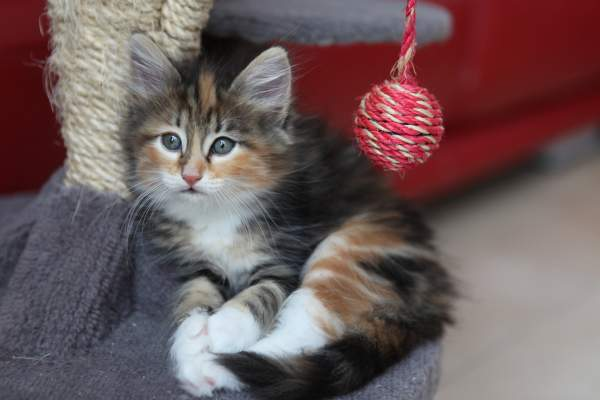
\includegraphics[width=8cm]{figures/kitten.jpg}
    \caption{挿入されたJPG画像}
    \label{fig:jpg}
\end{figure}
これは子猫です。

\section{SVG画像の挿入}
ことなるパッケージを使うとSVG画像も挿入できます。

\begin{figure}[H]
    \centering
    \includesvg[width=8cm]{figures/python-logo.svg}
    \caption{挿入されたSVG画像}
    \label{fig:svg}
\end{figure}
これはPythonのロゴです。

\section{PDF画像の挿入}
PDF画像変換せずとも挿入できます。
\begin{figure}[H]
    \centering
    
\includegraphics[width=9cm, page=2]{figures/quick-guide-gplv3.pdf}
    \caption{挿入されたPDF画像}
    \label{fig:pdf1}
\end{figure}

\section{表の挿入}
表も挿入できます。
\begin{table}[H]
    \centering
    % Second version of table, with booktabs.
    \begin{tabular}{lccccl}
        \toprule
        名前 & 1回目 & 2回目 & 3回目 & 4回目 & 平均 \\
        \midrule
        田中 & 100   & 90    & 80    & 70    & 85   \\
        鈴木 & 80    & 70    & 60    & 50    & 65   \\
        佐藤 & 60    & 50    & 40    & 30    & 45   \\
        \bottomrule
    \end{tabular}
    \caption{Latexで表を作る}
    \label{tab:latex_table}
\end{table}
表\ref{tab:latex_table}はLatexで作成した表です。